%%% cabecalho %%%
\documentclass[brazilian,12pt,a4paper,final]{article}
\usepackage[brazil]{babel}% *babel* contem as regras de ifenização
%\usepackage{t1enc}% *t1enc* permite o reconhecimento dos acentos do teclado
\usepackage[utf8]{inputenc}% permite reconhecimento automático de acentuação.
\usepackage{graphicx} % para incluir figuras em formato eps 
%ou
%\usepackage[pdftex]{graphicx}% para produzir PDF diretamente
\usepackage{color} % fontes soloridas
%%% fim do cabecalho %%%

\pagestyle{empty}
\title{Métodos Computacionais da Física A \\ Trabalho 15}
\author{Aluno: Átila Leites Romero \\ Matrícula: 144679 \\ IF-UFRGS}

\begin{document}
\maketitle

\section{}
\begin{quote}
1)Entenda o que acontece durante dentro do comando ``do .. while''. Qual é a vantagem de ler um arquivo desta maneira?
\end{quote}
A vantagem é que o programa se torna capaz de receber arquivos com
qualquer número de linhas.

\section{}
\begin{quote}
2)Você dispõe de 6 arquivos no moddle (estão colocados no link arquivos com os pontos a serem interpolados). Cada um deles corresponde a pontos da função seno entre 0 e 6, mas cada um tem um número diferente de pontos.
Primeiramente desenhe todos estes arquivos usando gnuplot . Use apenas pontos.

3) para cada um destes arquivos, calcule o valor da interpolação. Ou seja, use x entre 0 e 6. Faça isto por exemplo variando x de 0.1 em 0.1. Guarde estes pontos em um arquivo de saída.

4) desenhe compare os arquivos obtidos no item anterior com os arquivos que foram fornecidos. Gere uma figura em eps que tenha legendas e que seja clara (se precisar retirar algumas curvas para deixá-la mais clara, tire.)
\end{quote}

\begin{figure}[htbp]
\begin{center}
\rotatebox{-90}{\resizebox{8.0cm}{!}{\includegraphics{2.dat.eps}}}
\caption{2 pontos}
\label{fig_rotacao}
\end{center}
\end{figure}

\begin{figure}[htbp]
\begin{center}
\rotatebox{-90}{\resizebox{8.0cm}{!}{\includegraphics{4.dat.eps}}}
\caption{4 pontos}
\label{fig_rotacao}
\end{center}
\end{figure}

\begin{figure}[htbp]
\begin{center}
\rotatebox{-90}{\resizebox{8.0cm}{!}{\includegraphics{8.dat.eps}}}
\caption{8 pontos}
\label{fig_rotacao}
\end{center}
\end{figure}

\begin{figure}[htbp]
\begin{center}
\rotatebox{-90}{\resizebox{8.0cm}{!}{\includegraphics{16.dat.eps}}}
\caption{16 pontos}
\label{fig_rotacao}
\end{center}
\end{figure}

\begin{figure}[htbp]
\begin{center}
\rotatebox{-90}{\resizebox{8.0cm}{!}{\includegraphics{32.dat.eps}}}
\caption{32 pontos}
\label{fig_rotacao}
\end{center}
\end{figure}

\begin{figure}[htbp]
\begin{center}
\rotatebox{-90}{\resizebox{8.0cm}{!}{\includegraphics{64.dat.eps}}}
\caption{64 pontos}
\label{fig_rotacao}
\end{center}
\end{figure}

\section{}
\begin{quote}
5) Coloque o gráfico gerado no item 4 num arquivo .tex e responda como você interpreta o que está acontecendo.
Para ajudá-lo a responder esta questão, leia o final da página da complewiki,na parte de Fóruma de Lagrange.
Procure também no google o conceito de ``overfitting'' ou ``sobreajuste''.
\end{quote}
Com muitos pontos, começam a aparecer anomalias nas extremidades do gráfico,
porque o polinômio que o algoritmo encontra é de ordem muito elevada.
Já com muito poucos pontos, o algoritmo não encontra uma boa estimativa.

\section{}
\begin{quote}
6) Use o mesmo programa e os arquivos de entrada com 16 e 32 pontos para calcular o valor da função em pontos que estão fora do intervalo [0,6]. Calcule o valor da função entre [0,10] fazendo x variar de 1 em 1. Desenhe estas 2 curvas no gnuplot, comparando com a função sin(x) do gnuplot.
O que ocorre? Para qual caso a previsão (a extrapolação) é melhor, quando N=16 ou 32 ? 
\end{quote}

\begin{figure}[htbp]
\begin{center}
\rotatebox{-90}{\resizebox{8.0cm}{!}{\includegraphics{16b.dat.eps}}}
\caption{16 pontos}
\label{fig_rotacao}
\end{center}
\end{figure}

\begin{figure}[htbp]
\begin{center}
\rotatebox{-90}{\resizebox{8.0cm}{!}{\includegraphics{32b.dat.eps}}}
\caption{32 pontos}
\label{fig_rotacao}
\end{center}
\end{figure}

As duas extrapolações são muito ruins, quando passam de 6 saem completamente
do resultado esperado.

\end{document}
